
\subsection{Editing an Existing Account}

The Edit Account screen enables users to edit existing accounts that were previously added. Its layout is and functionality is similar to the Add Account screen, but users can now set an existing account as default, or delete an account through this screen. Note that accounts that have been marked as default cannot be deleted or set as default once again. 

\subsubsection{Application Screenshots}
\begin{figure}[h]
 
\begin{subfigure}{0.5\textwidth}
  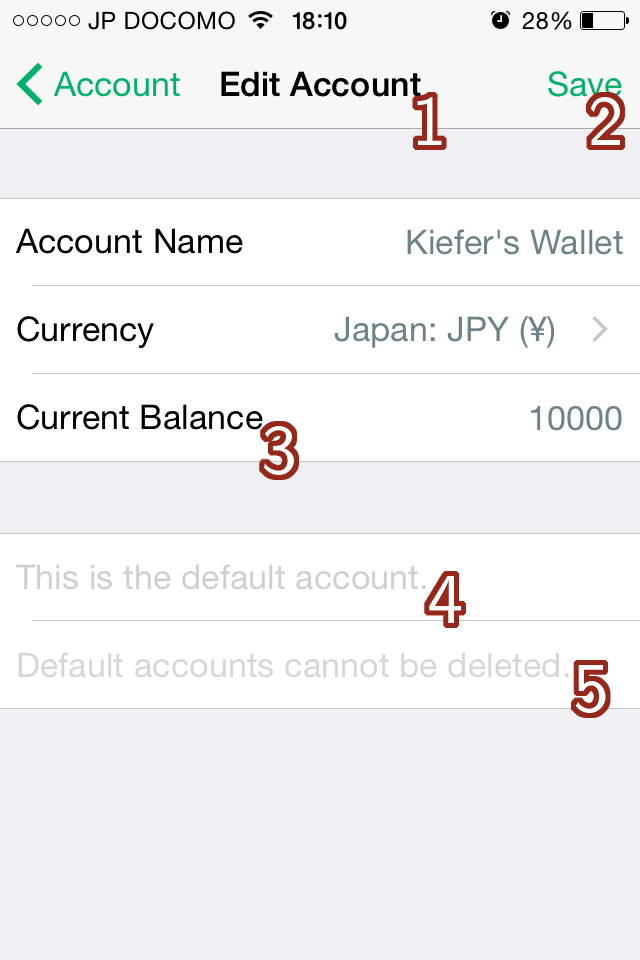
\includegraphics[scale=0.35]{ACC-0003-1} 
  \caption{Editing a Default Account}
  \label{fig:edit-account-1}
\end{subfigure}
\begin{subfigure}{0.5\textwidth}
  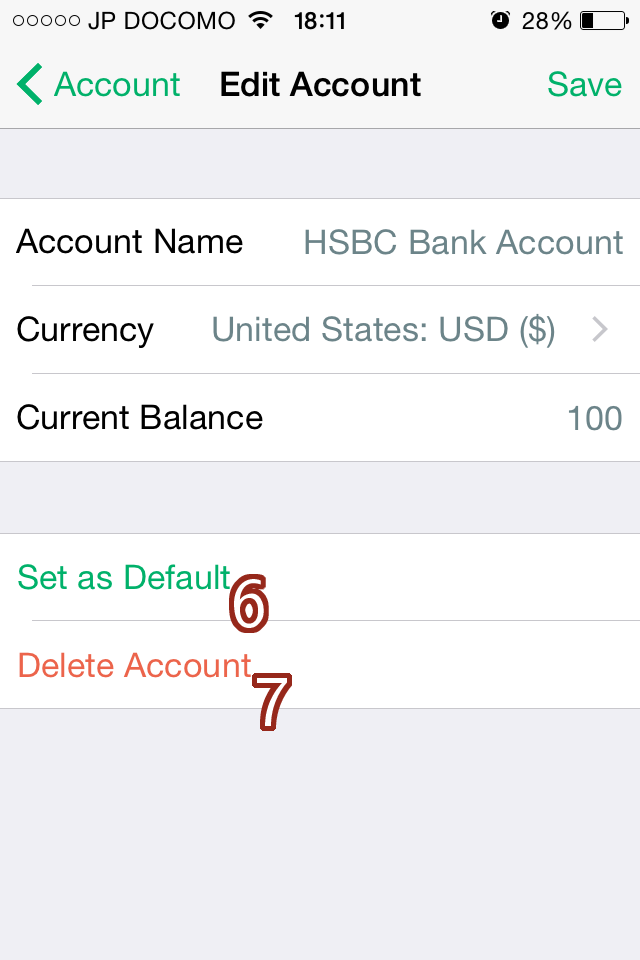
\includegraphics[scale=0.35]{ACC-0003-2}
  \caption{Editing a Non-Default Account}
  \label{fig:edit-account-2}
\end{subfigure}
\caption{Edit Account Screenshots}
\end{figure}

\screentable{
	\header{Screen Component}
    	{Type}
        {Description}
    \row{1. Screen Title}
    	{Label Title}
        {Localization Key: MENULABEL\_EDIT\_ACCOUNT}
    \row{2. Save Button}
    	{Button}
        {This button has the same functionality as the Done Button (Section 4.1), but it updates the core data instead of adding a new entry. \doublenewline
        Localization Key: BUTTON\_SAVE
        } 
    \row{3. Current Balance Cell}
    	{Table Cell}
        {This cell functions is similar to the Initial Balance cell in Section 4.1, but it has its localization key changed. \doublenewline
        
        Localization Keys: LABEL\_CURRENT\_AMOUNT
        } 
    \row{4. Disabled Default Account Button}
    	{Button}
        {This button cannot be tapped, and it informs the user that the current account is marked as default.\doublenewline 
        
        Localization Key: BUTTON\_DEFAULT \_ACCOUNT\_MESSAGE
        } 
    \row{5. Disabled Delete Account Button}
    	{Button}
        {This button cannot be tapped, and it informs the user that it is not possible to delete default accounts.\doublenewline 
        
        Localization Key: BUTTON\_DEFAULT \_ACCOUNT\_DESCRIPTION
        } 
}

\screentable{
	\header{Screen Component}
    	{Type}
        {Description}
    \row{6. Set as Default Button}
    	{Button}
        {Once this button is tapped, it will mark the account as default, and will be disabled, turning into a state seen in the fourth item of this screen.\doublenewline 
        
        Localization Key: BUTTON\_SET\_AS\_DEFAULT	
        }  
	\row{7. Delete Button}
    	{Button}
        {Once this button is tapped, it will display a warning, telling the user that the action cannot be undone, as seen in Section 4.5.\doublenewline 
        
        Localization Key: BUTTON\_DELETE\_ACCOUNT	
        }  
}

\subsubsection{Use Cases}
